\documentclass[12pt]{article}

\usepackage{amsmath}
\usepackage{amsfonts}
\usepackage{float}
\usepackage{fancyhdr}
\usepackage{graphicx}
\usepackage[colorlinks=true,linkcolor=blue, citecolor=red]{hyperref}
\usepackage{url}
\usepackage[top=1in, left=.5in, right=.5in]{geometry}
\usepackage[utf8]{vietnam}
\usepackage{biblatex}
\usepackage{listings}
\usepackage{xcolor}
\lstset { %
    language=C++,
    backgroundcolor=\color{black!5}, % set backgroundcolor
    basicstyle=\footnotesize,% basic font setting
}


\addbibresource{main.bib}
\setlength{\headheight}{29.43912pt}
\addtolength{\topmargin}{-17.43912pt}

\pagestyle{fancy}
\lhead{
	Lab 03 - Thực nghiệm về bài toán sắp xếp tăng
}
\rhead{
    Trường Đại học Khoa học Tự nhiên - ĐHQG HCM\\
    CSC14007
}
\lfoot{\LaTeX\ by \href{https://github.com/trhgquan}{Trần Hoàng Quân}}

\title{
	CSC14007 - Nhập môn Phân tích độ phức tạp thuật toán\\
	Lab 03 - Thực nghiệm về bài toán sắp xếp tăng
}
\author{Trần Hoàng Quân - MSSV: 19120338}

\begin{document}
\maketitle
\tableofcontents
\pagebreak

\section{Thuật toán sinh mảng ngẫu nhiên với các phần tử phân biệt}
Với \texttt{longint} là macro của kiểu số nguyên 64 bit \texttt{int64\_t}. Thuật toán sinh mảng ngẫu nhiên được em cài đặt như sau:
\begin{figure}[H]
\centering
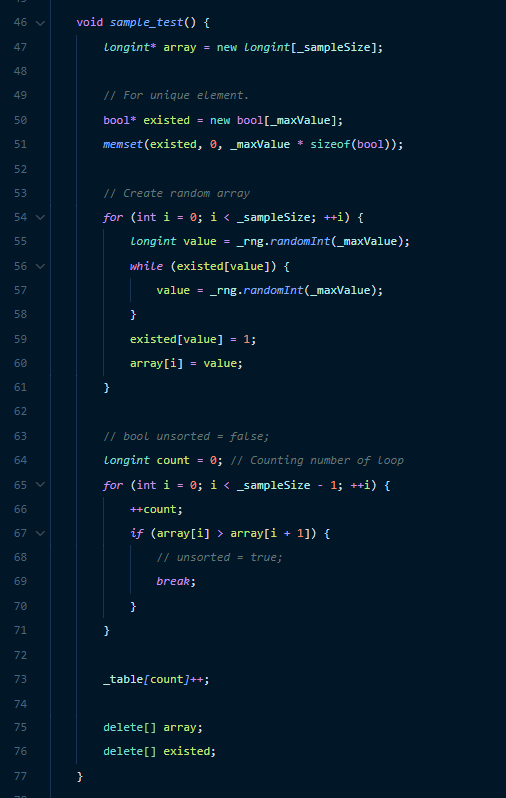
\includegraphics{testing-code.PNG}
\end{figure}

Ở row 75, \texttt{\_table} là một \texttt{std::map<longint, double>} lưu \texttt{key} là biến $X$ - số lần lặp, \texttt{value} là số lần xuất hiện của biến $X$. Em sẽ có một hàm tính kỳ vọng của bảng \texttt{\_table}, được cài đặt như sau:
\begin{figure}[H]
\centering
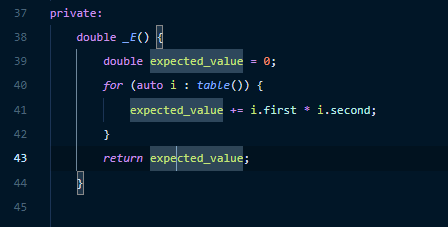
\includegraphics{private-e.PNG}
\end{figure}
Method \texttt{table()} ở dòng 40 được cài đặt để chuyển số lần xuất hiện thành tần số (chia cho tổng số phép thử đã thực hiện):
\begin{figure}[H]
\centering
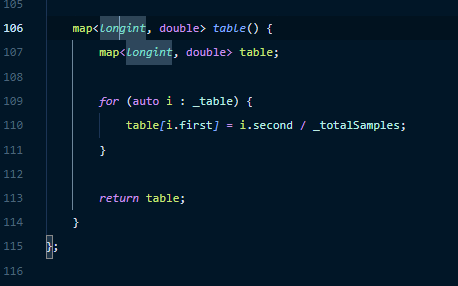
\includegraphics{table-method.PNG}
\end{figure}
Toàn bộ class \texttt{Testing} có thể được bố trí như sau:
\begin{lstlisting}
#define longint int64_t

class Testing {
private:
    RandomGenerator<longint> _rng;
    longint _totalSamples;
    longint _maxValue;
    longint _sampleSize;
    map<longint, double> _table;

private:
    /**
     * @brief Expected value of _table.
     * 
     * @return double 
     */
    double _E() {
        double expected_value = 0;
        for (auto i : table()) {
            expected_value += i.first * i.second;
        }
        return expected_value;
    }

    /**
     * @brief Testing samples.
     * 
     */
    void sample_test() {
        longint* array = new longint[_sampleSize];

        // For unique element.
        bool* existed = new bool[_maxValue]();

        // Create random array
        for (int i = 0; i < _sampleSize; ++i) {
            longint value = _rng.randomInt(_maxValue);
            while (existed[value]) {
                value = _rng.randomInt(_maxValue);
            }
            existed[value] = 1;
            array[i] = value;
        }

        // bool unsorted = false;
        longint count = 0; // Counting number of loop
        for (int i = 0; i < _sampleSize - 1; ++i) {
            ++count;
            if (array[i] > array[i + 1]) {
                // unsorted = true;
                break;
            }
        }

        _table[count]++;

        delete[] array;
        delete[] existed;
    }

public:
    /**
     * @brief Construct a new Testing object
     * 
     * @param totalSamples 
     * @param sampleSize 
     * @param maxValue 
     */
    Testing(longint totalSamples, longint sampleSize, longint maxValue) {
        if (sampleSize > maxValue) {
            throw "maxValue should be greater or equals sampleSize";
        }

        _totalSamples = totalSamples;
        _maxValue = maxValue;
        _sampleSize = sampleSize;

        // Perform test.
        for (int i = 0; i < _totalSamples; ++i) {
            cout << "Testing " << i + 1 << endl;
            sample_test();
        }
    }

    double E() {
        return _E();
    }

    /**
     * @brief Transform probability _table with counts to frequency.
     * 
     * @return map<longint, double> 
     */
    map<longint, double> table() {
        map<longint, double> table;

        for (auto i : _table) {
            table[i.first] = i.second / _totalSamples;
        }

        return table;
    }
};
\end{lstlisting}
Class \texttt{RandomGenerator} được cài đặt như sau, chủ yếu để generate random trong đoạn $[0, n -1 ]$:
\begin{lstlisting}
template<class T>
class RandomGenerator {
private:
    bool _seed = false;

public:
    T randomInt() {
        if (!_seed) {
            srand(time(NULL));
            _seed = true;
        }

        return rand();
    }

    T randomInt(T right) {
        return randomInt() % right;
    }

    T randomInt(T left, T right) {
        return (randomInt() % (left - right + 1)) + left;
    }
};
\end{lstlisting}
Hàm \texttt{main} được cài đặt như sau:
\begin{lstlisting}
int main() {
    try {
        // Testing a(1000000, 420, 1000);
        Testing a(so_sample, kich_thuoc_mang, phan_tu_max);
            
        cout << "Probability distribution (X f):" << endl; 

        for (auto i : a.table()) {
            cout << i.first << ' ' << i.second << endl;
        }

        cout << "Expected value = " << a.E() << endl;
    } catch (const exception& e) {
        cout << e.what() << endl;
    }
    

    return 0;
}
\end{lstlisting}
\section{Kết quả một số trường hợp đã khảo sát}
Em chọn kích thước mẫu là $10^6$ (sinh $10^6$ mảng). Kết quả kiểm thử như sau:
\subsection{n = 50, m = 100}
\begin{figure}[H]
\centering
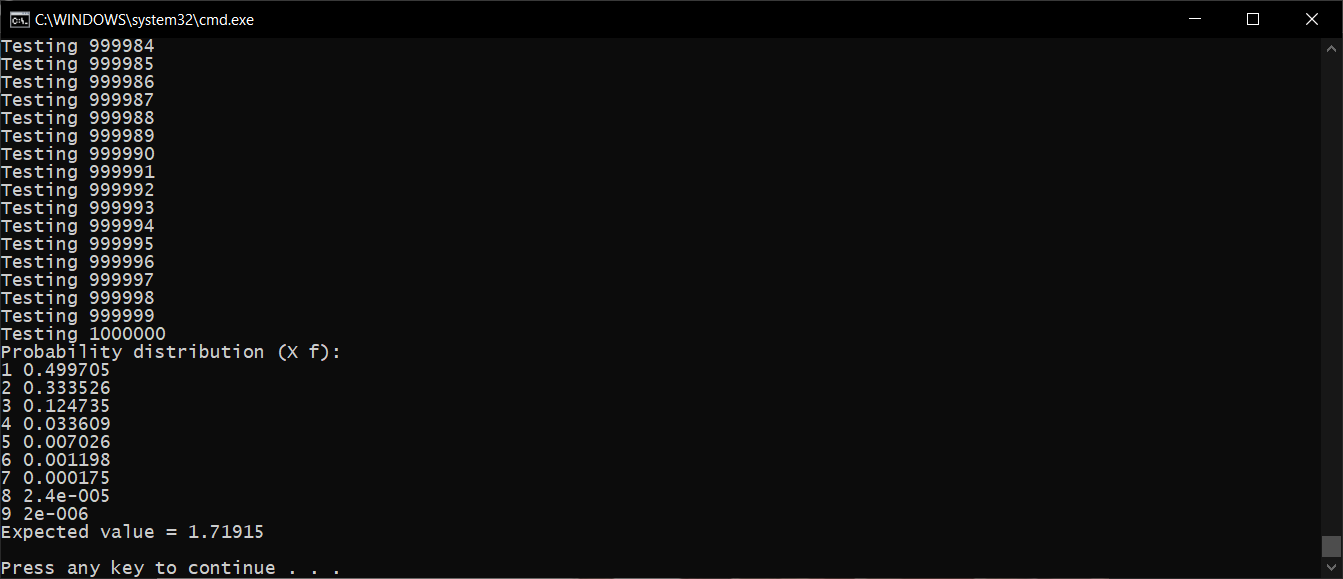
\includegraphics[scale=0.5]{50-100-1000k.PNG}
\end{figure}
\subsection{n = 100, m = 100}
\begin{figure}[H]
\centering
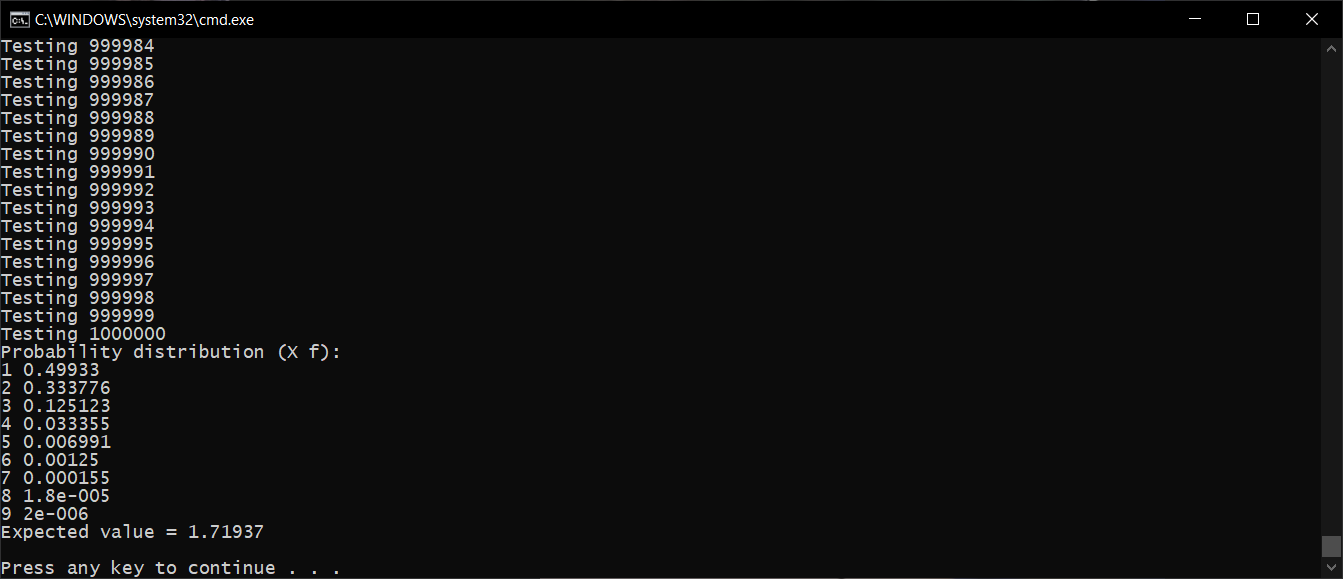
\includegraphics[scale=0.5]{100-100-1000k.PNG}
\end{figure}
\subsection{n = 200, m = 1000}
\begin{figure}[H]
\centering
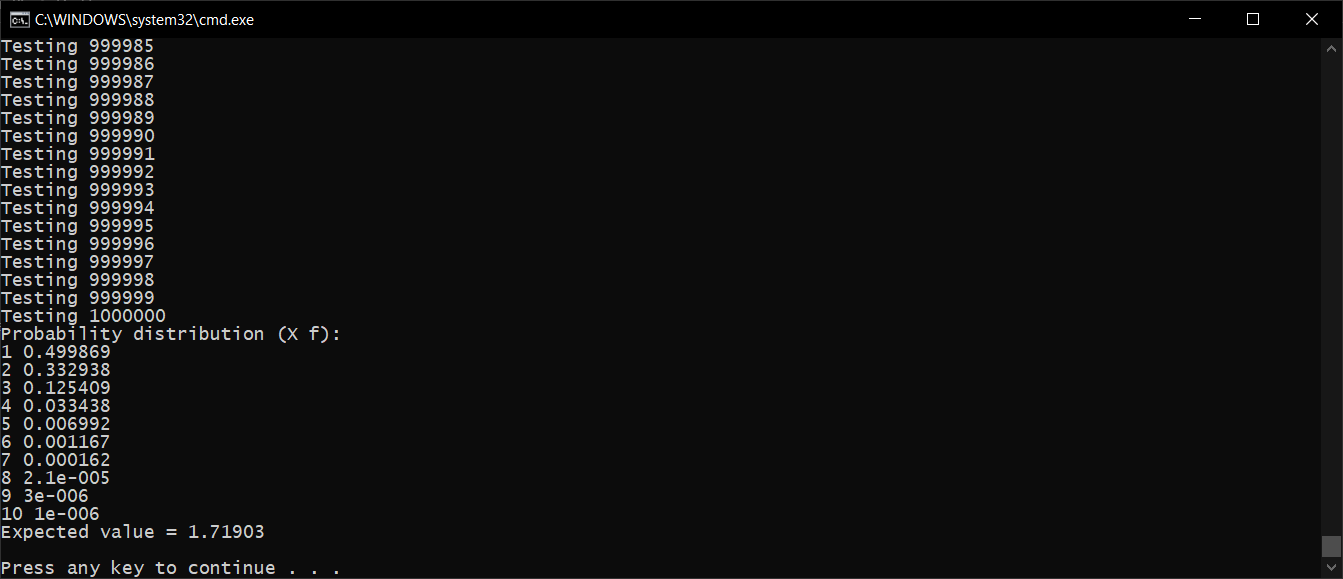
\includegraphics[scale=0.5]{200-1000-1000k.PNG}
\end{figure}
\subsection{n = 420, m = 1000}
\begin{figure}[H]
\centering
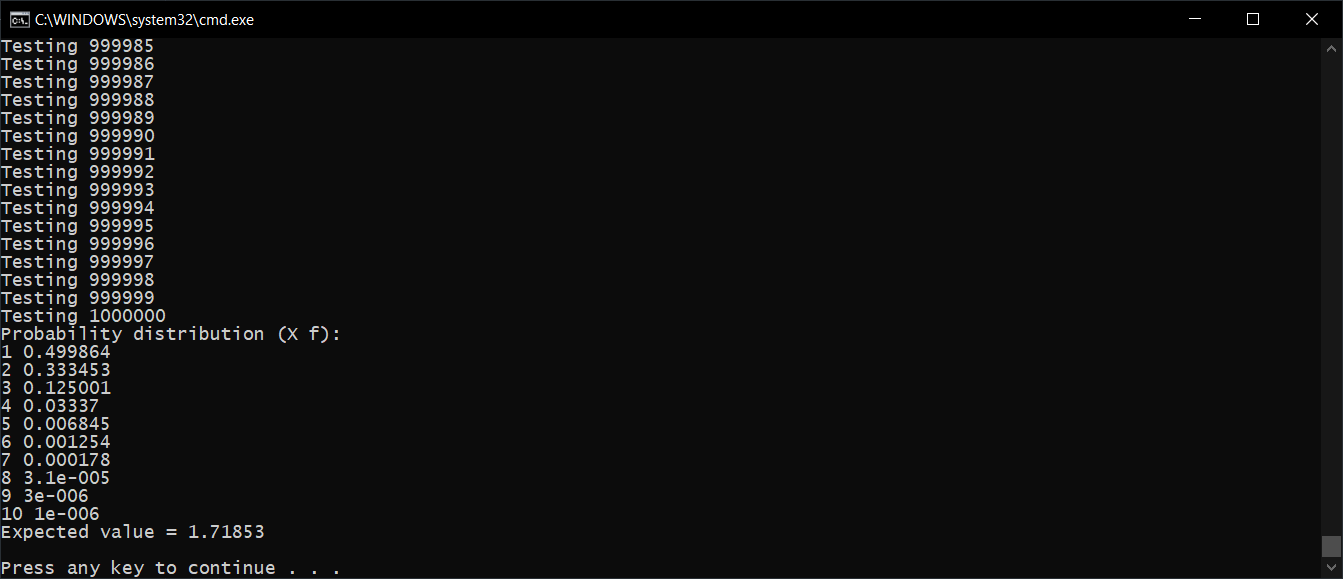
\includegraphics[scale=0.5]{420-1000-1000k.PNG}
\end{figure}
\subsection{n = 500, m = 1000}
\begin{figure}[H]
\centering
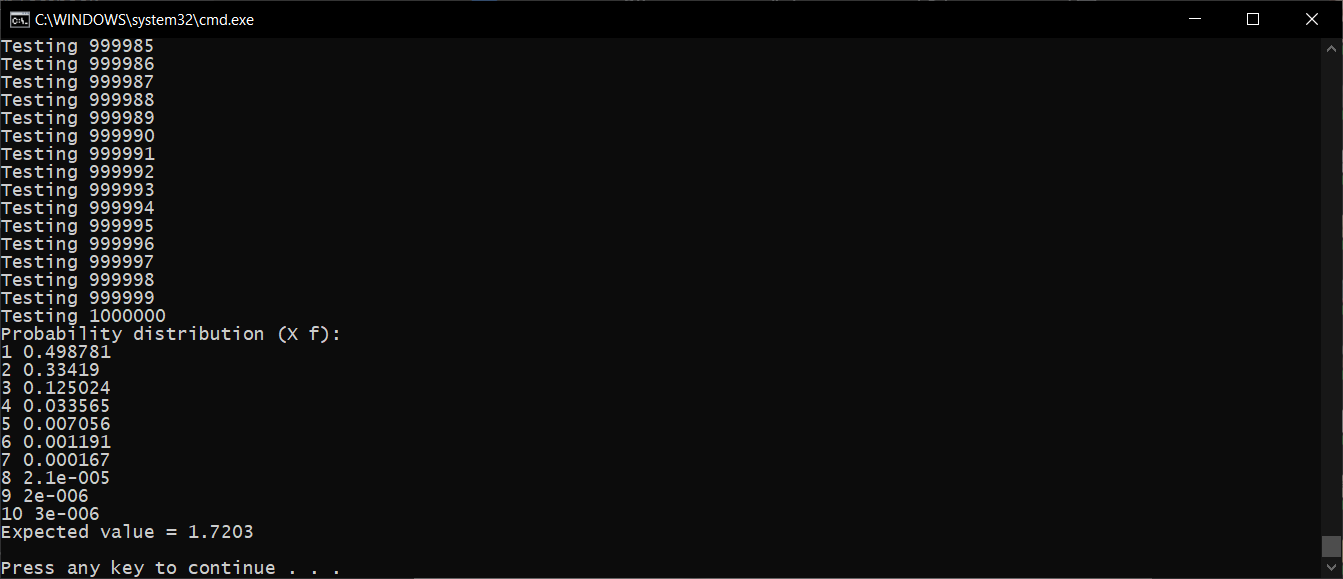
\includegraphics[scale=0.5]{500-1000-1000k.PNG}
\end{figure}
\subsection{n = 690, m = 1000}
\begin{figure}[H]
\centering
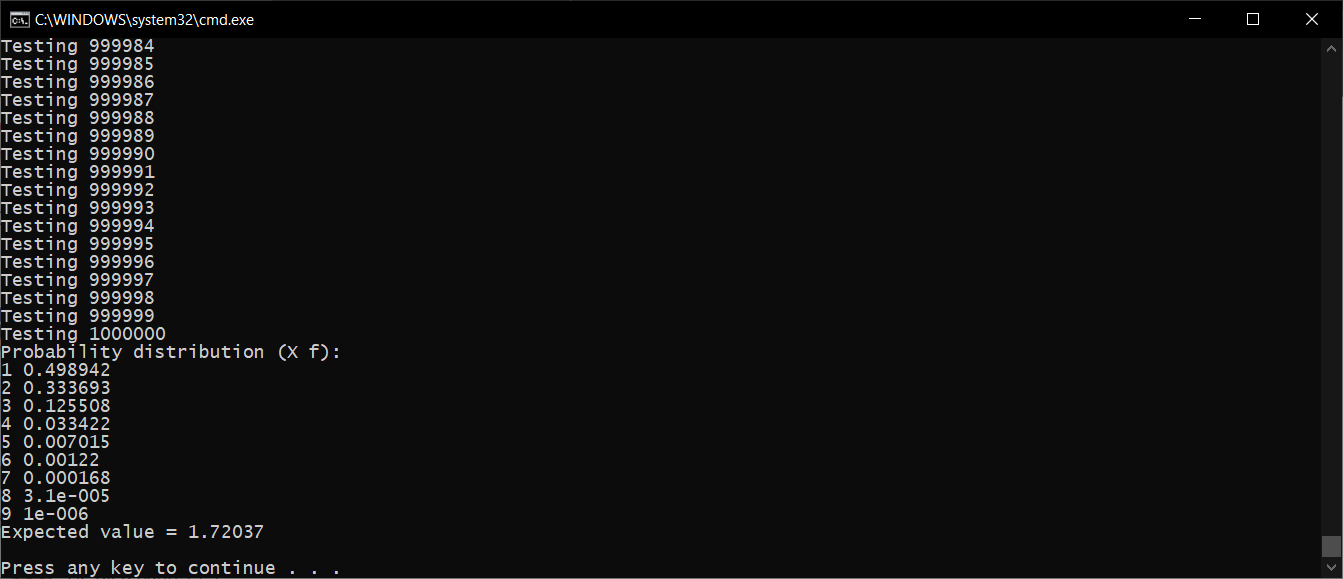
\includegraphics[scale=0.5]{690-1000-1000k.PNG}
\end{figure}
\subsection{n = 1000, m = 1000}
\begin{figure}[H]
\centering
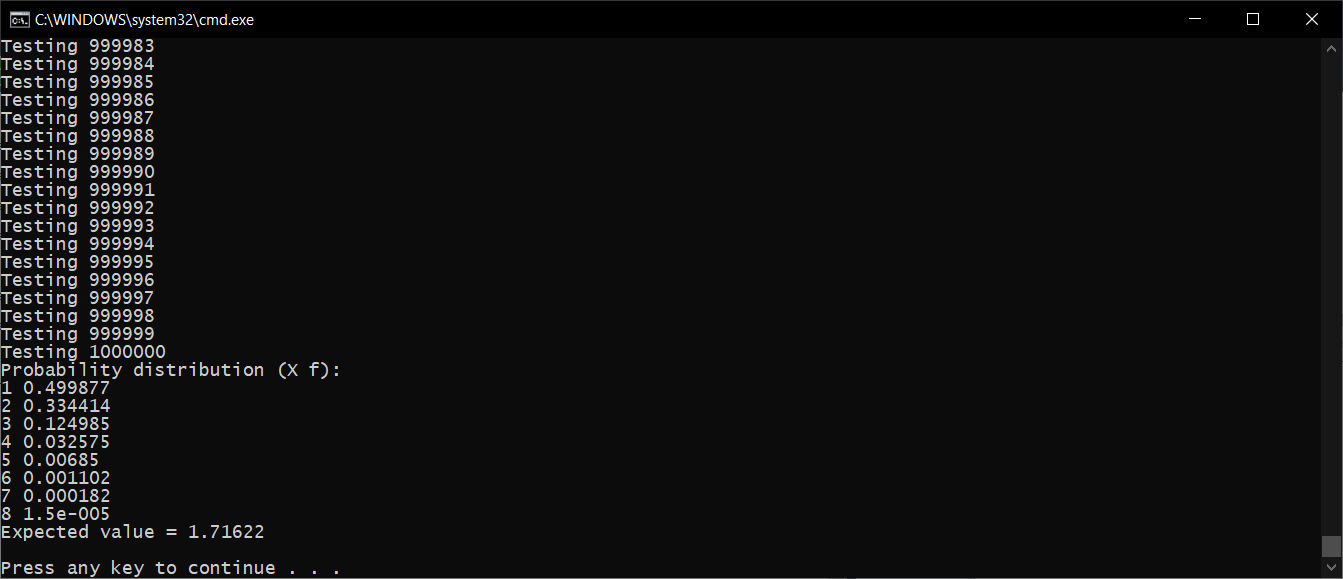
\includegraphics[scale=0.5]{1000-1000-1000k.PNG}
\end{figure}
\subsection{n = 2500, m = 10000}
\begin{figure}[H]
\centering
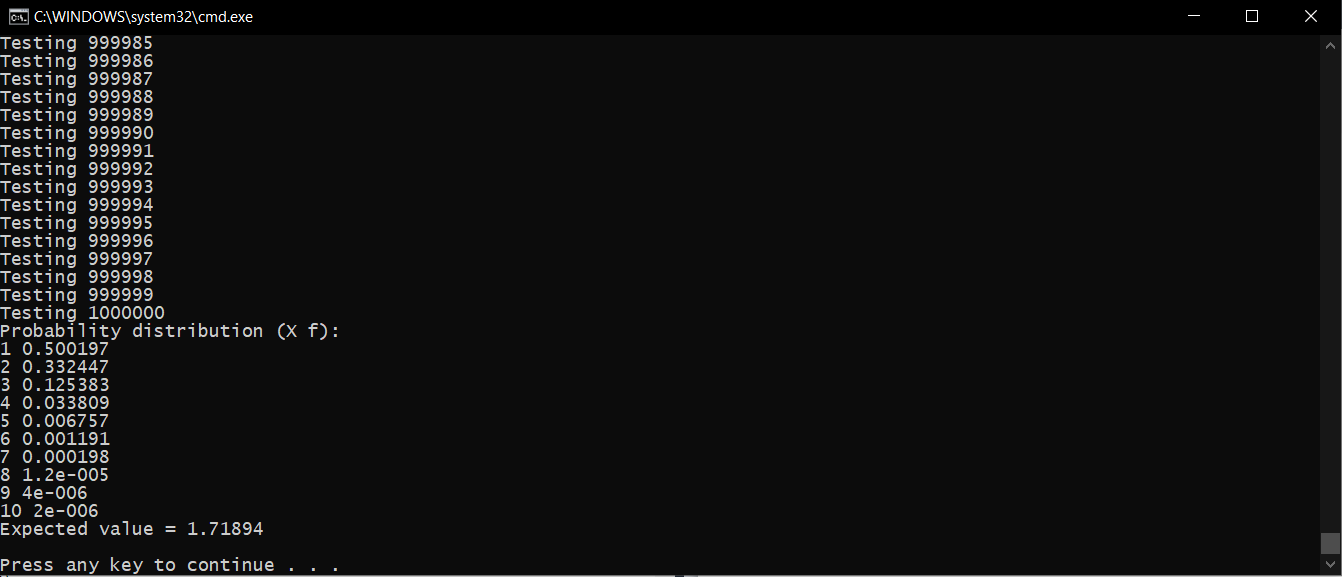
\includegraphics[scale=0.5]{2500-10k-1000k.PNG}
\end{figure}
\subsection{n = 5000, m = 10000}
\begin{figure}[H]
\centering
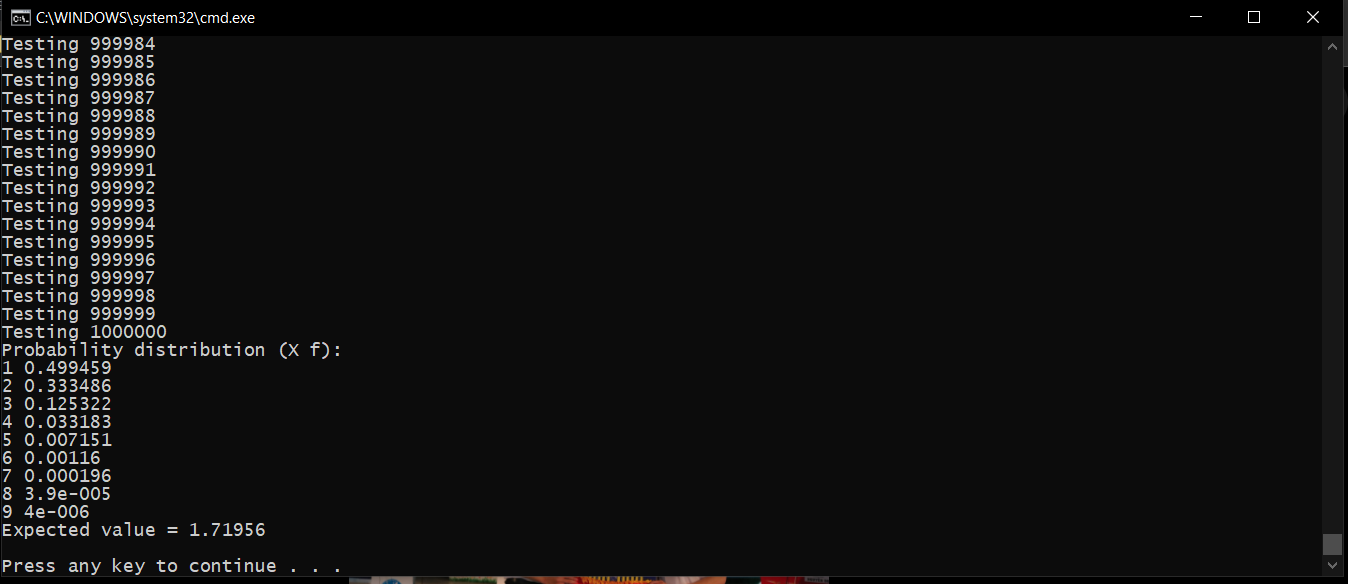
\includegraphics[scale=0.5]{5000-10k-1000k.PNG}
\end{figure}
\subsection{n = 6900, m = 10000}
\begin{figure}[H]
\centering
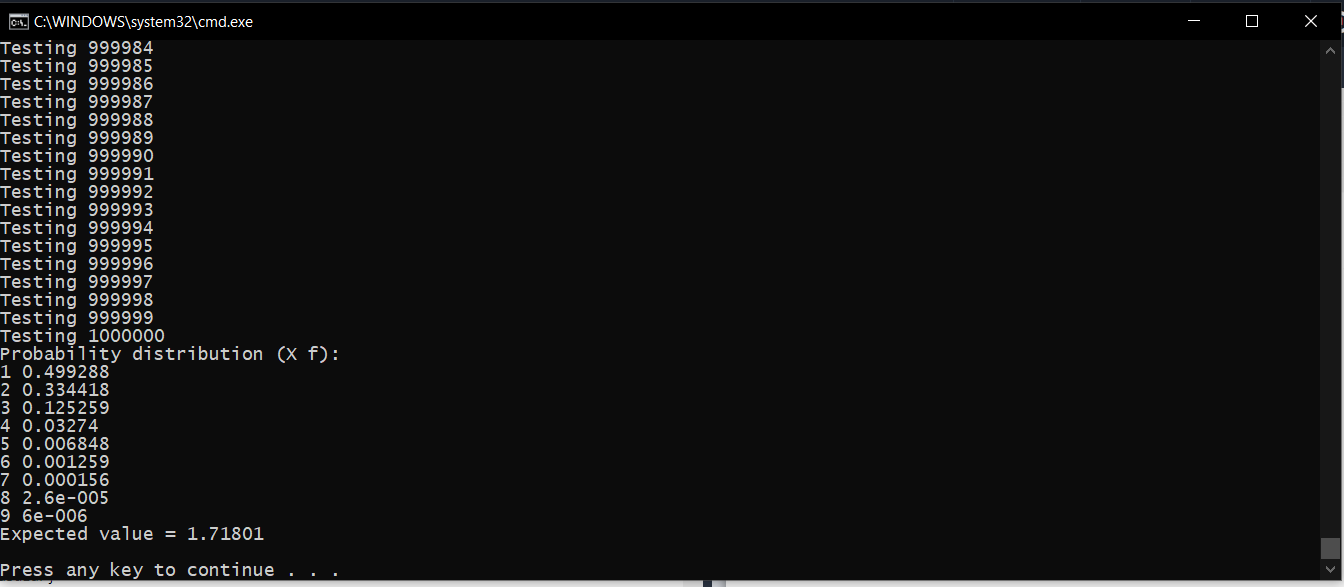
\includegraphics[scale=0.5]{6900-10k-1000k.PNG}
\end{figure}
\section{Kết luận}
Kết quả các lần kiểm thử được tóm tắt trong bảng dưới đây:
\begin{table}[H]
\centering
\begin{tabular}{|c|c|c|}
    \hline
    $n$ (kích thước mảng) & $m$ (phần tử lớn nhất) & Kỳ vọng số lần lặp ($E$)  \\
    \hline
    50 & 100 & 1.71915\\
    100 & 100 & 1.71937\\
    200 & 1000 & 1.71903\\
    420 & 1000 & 1.71853\\
    500 & 1000 & 1.7203\\
    690 & 1000 & 1.72037\\
    1000 & 1000 & 1.71622\\
    2500 & 10000 & 1.71894\\
    5000 & 10000 & 1.71956\\
    6900 & 10000 & 1.71801\\
    \hline
\end{tabular}
\caption{Một vài trường hợp qua kiểm thử}
\end{table}
Qua đó, ta có thể thấy giá trị kỳ vọng của số lần lặp dần hội tụ về 1.72.
\end{document}